\chapter{\textsc{Solas}, A 3-D Laser Ray Trace and Cross-Beam Energy Transfer Model} \label{chap:SOLAS}



This chapter will describe the \textsc{Solas} code, a 3-D Laser ray tracing module implemented in the \ac{Rad-MHD} code \textsc{Chimera}.
The chapter begins with a discussion of why ray tracing is frequently used to model `long-pulse' lasers for \ac{HEDP} experiments and why the standard framework is inadequate to model \ac{LPIs}.
It will then go on to describe the ray-trajectory solver, electric-field reconstruction and \ac{CBET} components of the model in detail.
Discussion of the validity of the model components will be included.
The numerical methods will also be presented alongside an extensive set validation problems to verify the implementation.


%###############################################################################################################################
%###############################################################################################################################
%###############################################################################################################################
\section{Ray Tracing for Hydrodynamic Simulations of Fusion Plasmas}

Nanosecond length (`long-pulse') lasers are often used as an external energy source in the field of \ac{HEDP}, for example in laboratory-astrophysics experiments \cite{tzeferacos_laboratory_2018,fiuza_electron_2020,meinecke_strong_2022}, equation of state studies \cite{kritcher_measurement_2020,smith_ramp_2014} or \ac{ICF} implosions \cite{zylstra_burning_2022,slutz_high-gain_2012,williams_demonstration_2024}.
Experimental design and analysis for these experiments must often be supported with fluid \ac{Rad-MHD} simulations.
The laser must therefore be described in these codes by a theoretical framework that is both valid to the problem and computationally tractable.
The physical processes by which lasers interact with plasma is a result of microscopic couplings between the laser field and particles or plasma waves.
The detailed microphysics of these interactions are often studied using \ac{PiC} codes \cite{nguyen_cross-beam_2021} or wave-based solvers \cite{myatt_wave-based_2017}, typically for scales and durations of tens of micrometres and hundreds of picoseconds.
Coupling these tools directly to multidimensional hydrodynamic simulations, which are often used for millimetre and nanosecond scales, would usually be computationally intractable.

The \ac{GO} assumptions are often widely applicable for \ac{HEDP} laser-plasma interactions (validity discussed in detail for \ac{ICF} plasmas in section \ref{sec:model_appliciability}) and therefore ray-tracing offers a computationally tractable approach to modelling lasers in these experiments.
By assuming static hydrodynamic profiles (which is normally valid for the propagation time of light through the computational domain) a laser beam can be discretized into a bundle of rays and the ray equations can then be integrated along their path to solve for the trajectory of the light, assuming that refraction dominates over diffraction.
A discrete amount of power can also be given to each ray.
If there is a suitable model for the power-absorption rate, this can also be integrated along the ray to provide an energy source for the plasma.
In many laser-driven \ac{HEDP} experiments, frequency-doubled or -tripled lasers and long scale-length plasmas mean that \ac{IB} is the dominant deposition process \cite{schmitt_importance_2023,schmitt_importance_2023-1}.
There are well established models for \ac{IB} that are suitable for implementation in ray-tracing codes, because they only require knowledge of the local plasma conditions, which are easily accessible via interpolation from the hydrodynamic grid to rays \cite{huba_nrl_2013,johnston_correct_1973}.
The combination of the ray equations and \ac{IB} deposition therefore is the basis for the vast majority of laser-modules coupled to hydrodynamic codes.

In laser-driven \ac{ICF} experiments however, another class of interaction, \ac{LPIs} are vitally important to the energetics of the implosion.
For example \ac{CBET} leads to a zeroth-order correction to the energy deposited in direct-drive experiments at the OMEGA laser facility, reducing coupled power late in the implosion to $\sim 50\%$ \cite{colaitis_inverse_2021}.
\ac{LPIs} cannot be included in the simple framework described above because they are non-linear\footnote{Non-linear in this context means that the interaction involves the interaction of multiple light and plasma waves.} and reduced theoretical models of the interaction rely on knowledge of the electric field or intensity of the light \cite{randall_theory_1981}.
Implementation in a tracing code therefore necessitates a method by which the separate light waves can `talk' to each other.
For example, the \ac{CBET} code described in this chapter stores information for separate components of laser beams on a common grid which can then interact via the `pump-depletion iterations', described in section \ref{sec:pump_dep_iters}.
Additionally, the knowledge of electric field or intensity is problematic because this is not an attribute which standard \ac{GO} rays posses.
Heuristically, rays have an associated power, so an area is required to obtain an intensity.
The evolution of a portion of the beam front's area is governed by a first order expansion of the Helmholtz equation, rather than the zeroth order expansion which is most commonly used in ray-tracing packages for hydrodynamic codes \cite{colaitis_towards_2014}.
The first order expansion introduces an equation for the ray amplitude which can be solved in a variety of ways and used to obtain the electric field of the light.
Section \ref{sec:SOLAS_field_reconstruc} describes the approach taken to solving for the amplitude of the rays in \textsc{Solas}, which is to track the area of a triangle\footnote{For a 2D ray trace, a pair of rays is used rather than a triangle.} of rays around a standard \ac{GO} ray.

For direct-drive \ac{ICF} simulations, it is also desirable to have a 3D ray trace, where rays travel and refract in 3 dimensions.
In some computational direct-drive studies, particularly in 1D hydrodynamic simulations, simplified laser models are employed in which rays travel radially toward the target \cite{paddock_one-dimensional_2021}.
This simplification is can lead to significant deviations from reality, as it neglects any refractive losses, which become increasingly significant late in the implosion as the target converges.
Assuming that rays travel radially inward also leads to deposition occurring closer to the critical surface compared to a true 3D ray trace, leading to an overestimation of the drive.
The growth of \ac{LPIs} also depends on vector summations of light and plasma wavevectors, so a 3D ray trace is necessary when modelling these effects.
Predictive direct-drive simulations therefore necessitate a fully 3D ray-trace, even when coupled to just 1D hydrodynamics.


%###############################################################################################################################
%###############################################################################################################################
%###############################################################################################################################
\section{Existing Cross-Beam Energy Transfer Models}

There are a variety of existing computational tools used to model \ac{CBET} for \ac{ICF} conditions, which are used to study the interaction from first principles, reduced models to investigate the effect of \ac{CBET} when coupled to hydrodynamics or validation tools to test the implementation of these reduced models.
A non-exhaustive list will be presented here of existing codes, provided mainly as context for the work presented in this chapter.

%################################################################################
%################################################################################
\subsection{Ray Based Models}

The most common tool to study the coupling of \ac{CBET} effects into hydrodynamics are reduced ray-based models which use the linear gain theory of \ac{SBS}, outlined in section\ref{sec:SBS_linear_gain}.
There are a variety of different codes used to simulate this.
The main difference between the models is the way that the electric field or intensity of the laser light is obtained.

\paragraph*{\ac{IRT}} This is an approach, implemented within the \textsc{Ifriit} code, that creates a mapping between points on an initial beam front and arbitrary locations within the plasma \cite{colaitis_real_2019,colaitis_adaptive_2019}.
This is in contrast to \ac{FRT}, which is used in the other ray-based approaches listed below, where discrete points on the beam front are integrated forward to discrete points within the plasma.
\ac{IRT} is a very efficient approach for convex, approximately spherically symmetric plasma profiles, it can not deal well with beams that have multiple caustics\footnote{Caustics are defined and discussed in detail in section \ref{sec:SOLAS_ray_amplitude}.}, where the \ac{FRT} approach is better suited.
\textsc{Ifriit} has been coupled to the 3-D \ac{Rad-Hydro} code, \textsc{Aster} from \ac{LLE}, and prior to the development of \textsc{Solas}, \textsc{Aster}-\textsc{Ifriit} was the only code combination capable of conducting 3-D direct-drive simulations with in-line \ac{CBET} \cite{colaitis_inverse_2021}.

\begin{figure}[t!]
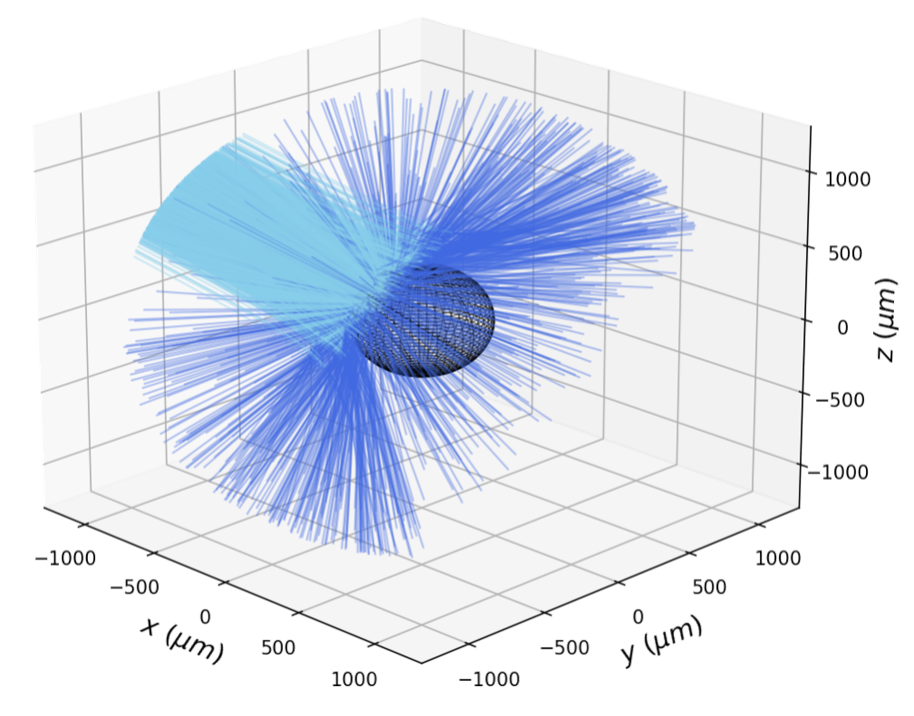
\includegraphics[width=10cm]{Numerics/Images/Reflected_Rays.png}
\centering
\caption{3D ray trajectories through a spherically symmetric, OMEGA direct-drive scale density profile.
The incident rays are plotted in cyan and the reflected rays, which spread out over a very large solid angle, are plotted in dark blue.
The critical density is represented by the black mesh.}
\label{fig:reflectedrays}
\end{figure}

\paragraph*{Ray Statistics Approach} The \textsc{Lasnex} \cite{strozzi_interplay_2017}, \textsc{Troll} \cite{liberatore_first_2023} and \textsc{Draco} codes \cite{marozas_wavelength-detuning_2018}, developed at \ac{LLNL}, \ac{CEA} and \ac{LLE} respectively, implement field-reconstruction methods which depend heavily on having many rays per computational cell.
\textsc{Lasnex} and \textsc{Troll}, used mainly for indirect-drive hohlraum simulations, obtains the intensity of light by first propagating rays through the mesh and obtaining the deposited power in each grid cell.
The intensity is then obtained from the power in each cell using electromagnetic energy conservation.
Obtaining the intensity from deposition means that the field cannot be reconstructed in vacuum regions where no deposition occurs.

\textsc{Draco} uses a similar approach, but the intensity is estimated by multiplying the ray power by the path length in a cell divided by the cell volume, which gives a dimensional estimate for the intensity.
Both of these approaches require many rays-per cell to accurately obtain the intensity, $\mathcal{O}(100)$ \cite{debayle_unified_2019}.
For direct-drive simulations this is extremely computationally expensive, because backscatter \ac{CBET} dominates over sidescatter, therefore the reflected field of each beam must be resolved, and each beam spreads out over a large solid angle after reflecting off a convex density profile, as is demonstrated in figure \ref{fig:reflectedrays}.
This means that orders of magnitude more rays are required than for approaches which can accurately obtain the field from a single ray per cell.

Another drawback of both of these approaches is that caustics of beams (regions where the amplitude of rays diverge) are not identifiable, and therefore fields cannot be capped to physically accurate, diffraction-limited values.
If a significant amount of \ac{CBET} occurs at caustics, such as in direct-drive \ac{ICF}, then erroneous global multipliers to \ac{CBET} gains must be applied which are effectively free parameters that must be tuned to obtain a pre-known reduction in absorbed energy.
This means that it is difficult to trust this approach for predictive direct-drive simulations.

\paragraph*{\ac{PCGO}} In this approach, each ray has an associated Gaussian intensity profile, the width of which is integrated along the ray trajectory \cite{colaitis_towards_2014,colaitis_crossed_2016}.
A single ray can be used per cell as each ray can have an intensity which is interpolated to the mesh, but the reconstructed field at caustics is not accurate and the width evolution is only valid for a short propagation distance.
This approach was coupled to the \textsc{Chic} 2 dimensional hydrodynamics code, but is difficult to extend to 3D as the implementation relied on interacting only rays whose centroids crossed, which does not generically occur in 3D for non-coplanar rays \cite{colaitis_modeling_2015}.

\paragraph*{Neighbouring Rays} The \textsc{BeamCrosser} code obtains an area for each ray by co-tracing a triangle of neighbouring rays around it that can be converted into a ray amplitude and therefore electric field from electromagnetic energy conservation \cite{edgell_mitigation_2017}.
Integrating the amplitude along the ray trajectory means that the caustics can be identified and therefore fields in those regions capped to diffraction limited values \cite{follett_ray-based_2018}.
Each ray also has an individual field value, and it is therefore less dependent on ray-per-cell statistics than geometric models, such as that used in the \textsc{Draco} code described above \cite{follett_validation_2022}.
Section \ref{sec:SOLAS_field_reconstruc} describes the implementation of this approach into the \textsc{Chimera} 3D \ac{Rad-MHD} code, which had not previously been used coupled to hydrodynamics in multidimensional simulations.


%################################################################################
%################################################################################
\subsection{Wave Solvers}

Solving Maxwell's equations with coupling to a plasma background is a useful tool for the study of \ac{LPIs}.
The main code used in the \ac{ICF} community that uses this approach is \textsc{Lpse}, which propagates light waves through a prescribed, spatially varying density, temperature and velocity profile in 1D$\rightarrow$3D \cite{myatt_wave-based_2017,myatt_lpse_2019}.
It then solves the nonlinear coupling of electromagnetic waves by allowing first order plasma perturbations (obtained from the ponderomotive beat pattern between light), which then feed back into the wave propagation.
The perturbative approach means that \textsc{Lpse} is limited to linear problems and the temporal and spatial resolution required to resolve the beat frequency mean that coupling to multidimensional \ac{Rad-Hydro} simulations is not feasible.
However, it is an extremely useful tool to validate implementation of \ac{CBET} models, especially in situations like scattering at laser caustics, such as the test case presented in section \ref{sec:SOLAS_CBET_caustic_test}.
It can also been used for many other important studies, such as the mitigation of \ac{LPIs} via laser bandwidth and the effect of beam smoothing techniques on the growth rate of \ac{LPIs} \cite{follett_thresholds_2021}.

%################################################################################
%################################################################################
\subsection{\ac{PiC} Codes}

Both Ray based codes and \textsc{Lpse} are ill-suited to the study of \ac{LPIs} in the non-linear regime, where the laser intensity becomes sufficiently large that the ponderomotive imprint on the plasma can no longer be treated perturbatively.
Understanding this growth and saturation of \ac{LPIs} in this regime is particularly important for \ac{ICF} schemes with high peak intensities, such as during the ignitor spike in shock ignition pulses \cite{perkins_shock_2009}.
Often kinetic effects such as ion-trapping become important in non-linear saturation, where ion are trapped and then accelerated in the \ac{CBET} induced \ac{IAW}, leading to changes in the \ac{IAW} phase velocity and therefore a loss of resonance \cite{nguyen_cross-beam_2021}.
\ac{PiC} codes are therefore well suited to model this kinetic saturation, albeit over short timescales and in simulations that are not truly representative of direct-drive conditions, due to computational expense \cite{seaton_cross-beam_2022-1}.
Kinetic modelling of \ac{CBET} has demonstrated that the growth of \ac{LPIs} can be a much more complex, time-dependent problem than is assumed by the linear-models used in ray-based codes, leading to larger net energy transfers \cite{seaton_cross-beam_2022}.

%###############################################################################################################################
%###############################################################################################################################
%###############################################################################################################################
\section{\textsc{Solas} 3-D Laser Ray Trace}

This section will describe how the ray equations, derived from the Helmholtz equation in section \ref{sec:ray_equations} are solved in the \textsc{Solas} module for the \textsc{Chimera} \ac{Rad-MHD} code.
Details of the mesh used for spherical simulations and load balancing options shall be provided as well as validation problems.

%################################################################################
%################################################################################
\subsection{Outline of \textsc{Solas}-\textsc{Chimera} Interfacing}

\begin{figure}[t!]
    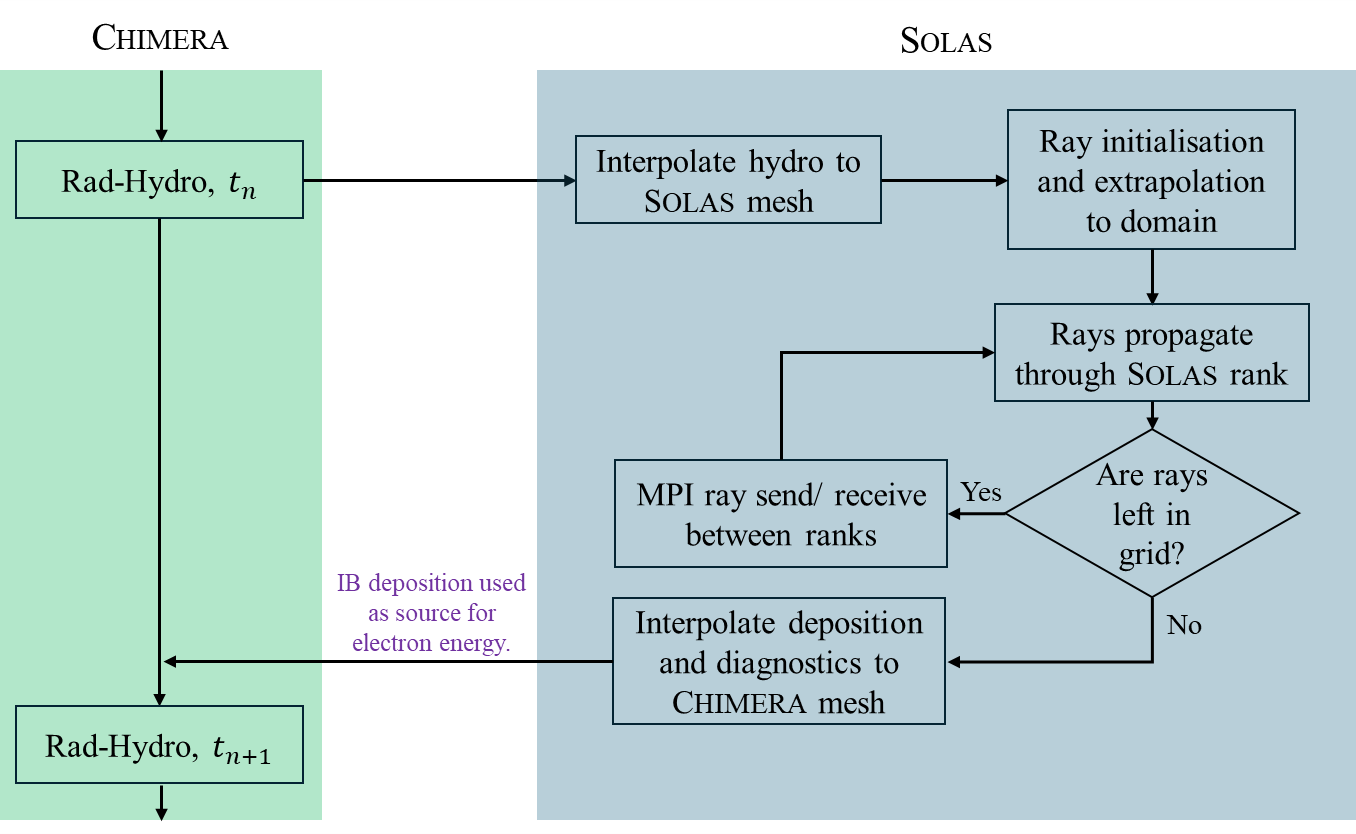
\includegraphics[width=8cm]{Numerics/Images/raytrace_flowchart.png}
    \centering
    \caption{A flowchart illustrating the basic interfacing between \textsc{Chimera} and \textsc{Solas}.
    The interpolation steps refer simultaneously to the re-domain balancing and cell combination procedures described in section \ref{sec:SOLAS_mesh}.}
    \label{fig:raytrace_flowchart}
\end{figure}

A simple flowchart for the basic \textsc{Solas} operational loop and the interfacing with \textsc{Chimera} is shown in figure \ref{fig:raytrace_flowchart}.
At the start of a \ac{Rad-Hydro} timestep, $t_n$, the hydrodynamic variables (stored on the Eulerian \textsc{Chimera} grid), which are necessary to compute ray trajectories and \ac{CBET} gains are interpolated to the \textsc{Solas} mesh.
Rays are then initialised on the beam port locations and extrapolated to the computational domain, before being traced through the grid.
\textsc{Solas} uses a \ac{MPI} domain balanced approach to parallelization, the reasons for which will be discussed in more detail in section \ref{sec:SOLAS_mesh}, therefore rays are traced up to the internal borders of the domain subsection used for the \ac{MPI} rank.
Rays are then passed between ranks and moved through their new subdomain until they exit the entire simulation domain.
As rays move through the domain, they contribute to total for \ac{inv-Brem} deposition in each grid cell and other computational diagnostics.
When all rays have exited the domain, the \textsc{Solas} quantities such as deposited energy which have been built up from the ray trace are then interpolated onto the \textsc{Chimera} grid, where the \ac{inv-Brem} deposition is used as a source term for the electron energy in the subsequent \ac{Rad-Hydro} step, $t_{n+1}$.
The interpolation, initialization and propagation steps will be outlined in sections \ref{sec:SOLAS_mesh}, \ref{sec:SOLAS_ray_init}, \ref{sec:SOLAS_ray_propagation} respectively.


%################################################################################
%################################################################################
\subsection{\textsc{Solas} Mesh Structure}
\label{sec:SOLAS_mesh}

For direct-drive \ac{ICF} simulations which model the laser using ray-tracing, especially those which include \ac{CBET}, the choice of an appropriate computational mesh on which to conduct the laser ray-trace is crucial to obtaining an accurate and noise-free energy deposition.
A well-chosen grid can also significantly reduce the run-time and memory requirements of the calculation.
The mesh used for hydrodynamic simulations of these experiments is often not well suited for ray-tracing calculations.
For example, hydrodynamic grid resolutions often have excessive resolution in the corona to resolve the gradients in the laser quantities, which greatly increases the expense of tracing rays through the mesh, without significantly enhancing the accuracy of the solution.
This section will describe the approach taken in the \textsc{Solas} code to create a grid structure which is well suited to direct-drive simulations which we have found to accurately resolve laser energy deposition both with and without \ac{CBET} in a memory-efficient manner.

%##################################################
\subsubsection{Re-Domain Balance for Radial Geometries}

\begin{figure}[t!]
    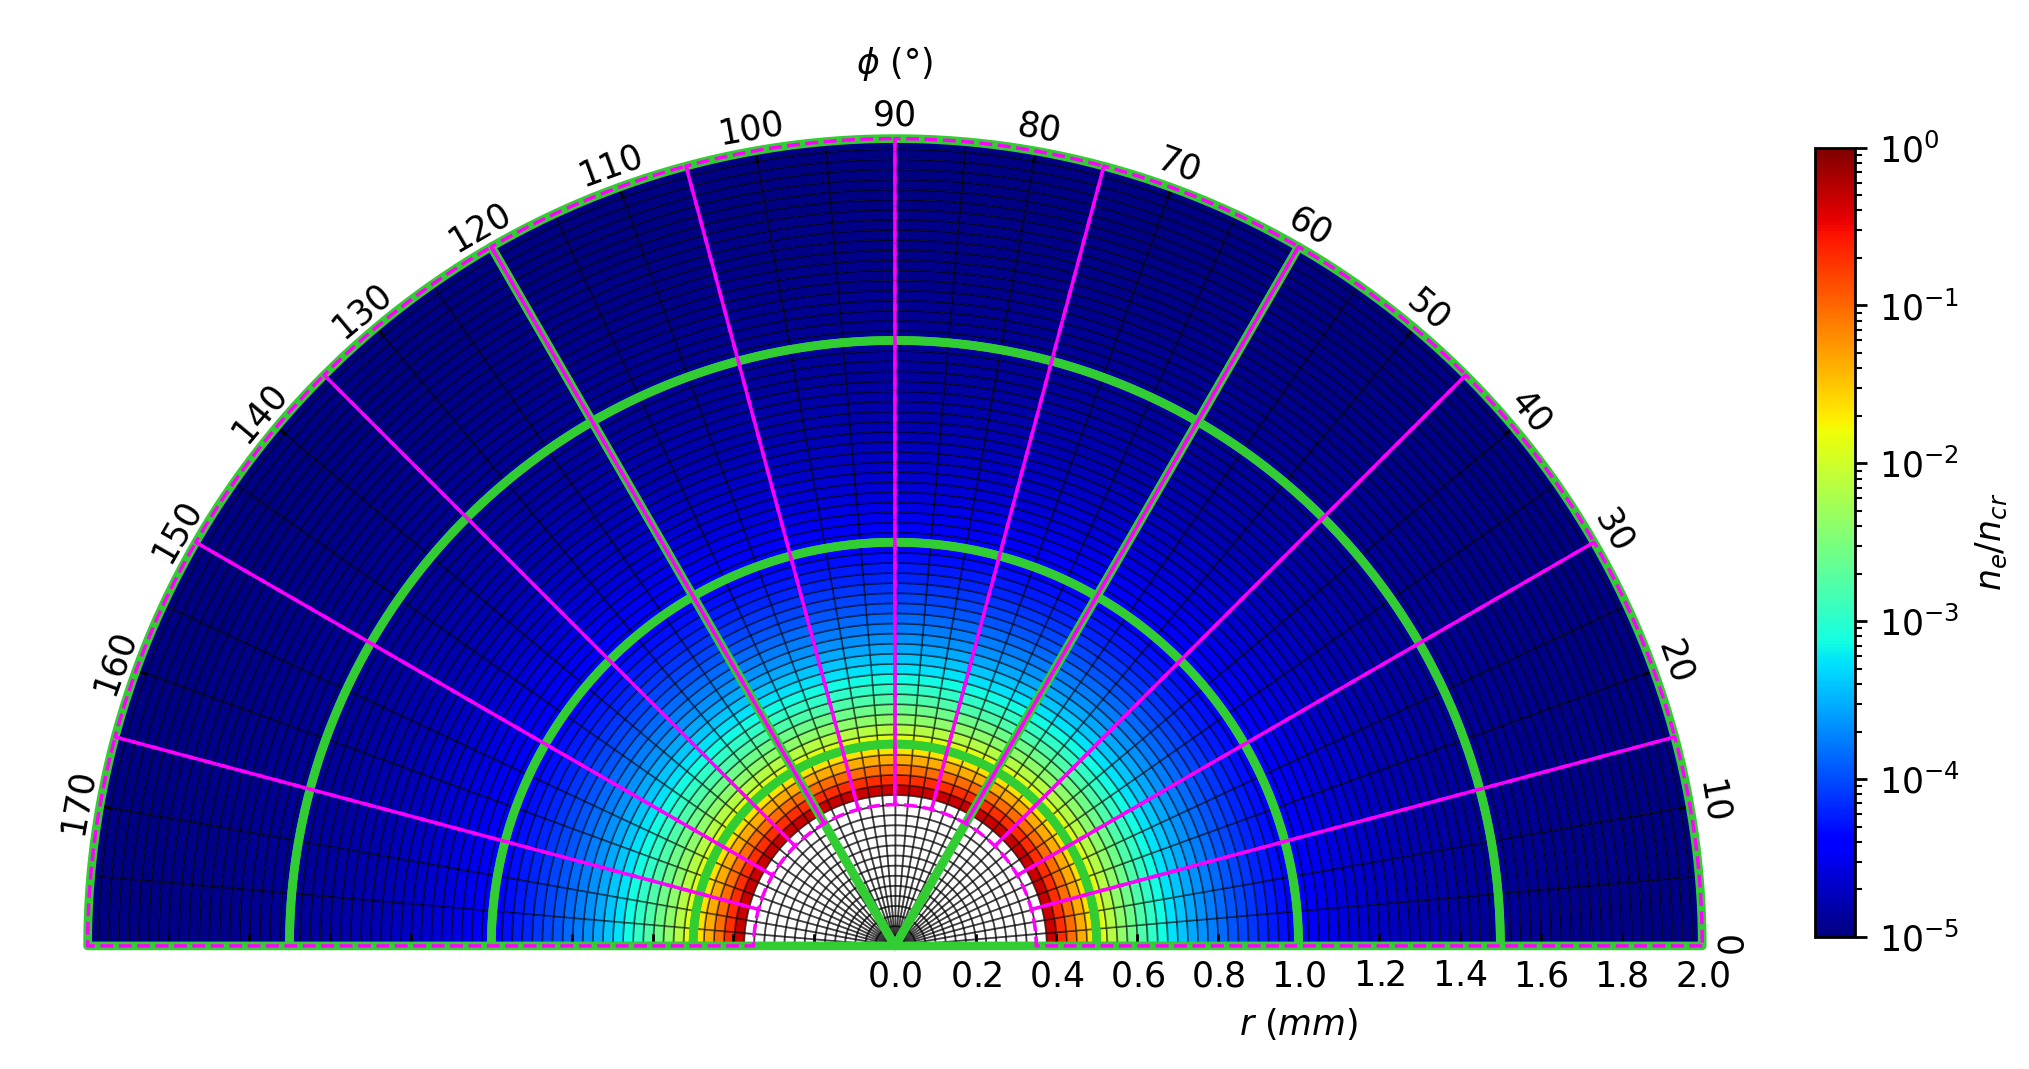
\includegraphics[width=16cm]{Numerics/Images/SOLAS_CHIMERA_domain.png}
    \centering
    \caption{An illustrative diagram demonstrating the MPI re-domain balanced grid employed by \textsc{Solas} compared to the \textsc{Chimera} domain balanced grid for a cylindrical geometry.}
    \label{fig:SOLAS_CHIMERA_domain}
\end{figure}

\ac{Rad-MHD} codes often employ a domain balanced approach to parallelization\footnote{This includes the \textsc{Chimera} code for which \textsc{Solas} has been developed.}, where each computational rank solves a portion of the entire spatial domain each discrete timestep.
Additional `ghost-cells' are stored in the subdomains and used to calculate gradients on the boundaries between ranks, which are updated with inter-rank communications each timestep.
The hydrodynamic grid for \textsc{Chimera} is Eulerian, with options for Cartesian, cylindrical or spherical-polar grids.

The optimal domain balancing minimises communication between ranks, which leads to cubic\footnote{Cubic in cell dimension, not necessarily in physical space for non-Cartesian geometries.} subdomains.
If computing a laser raytrace through this domain however for a typical direct-drive calculation however, initially rays travel approximately radially and therefore regularly encounter processor boundaries where they must be transferred between ranks.
A more optimal domain decomposition for the raytrace minimises radial splitting to avoid excessive passing of rays.
When required for spherical and cylindrical simulations, \textsc{Solas} therefore takes the hydrodynamic variables on the \textsc{Chimera} grid and re-domain balances the grid for the raytrace, such that the splitting does not occur in the radial coordinate.
An example of this re-domain balancing is shown in figure \ref{fig:SOLAS_CHIMERA_domain} for an illustrative cylindrical mesh.
The \textsc{Chimera} domain decomposition divides the radial and azimuthal extent into 4 and 3 respectively, whereas \textsc{Solas}' division is purely in the azimuthal direction.
For spherical and cylindrical direct-drive simulations where there is a defined, global minimum critical radius, \textsc{Solas}' mesh excludes the grid cells below this minimum radius beyond which the rays cannot reach in order to reduce the memory burden of the re-gridding.

An alternative approach to domain-decomposition parallelization of the module would be to use the \ac{OpenMP} package, where processors share memory across a computational node.
In this approach, the entire laser grid would be stored once on the shared memory of the node and separate ranks would trace rays through the entire domain without the need for transfers.
While this is certainly a preferable approach for a standard raytrace to the \ac{MPI} procedure described above, including a model for \ac{CBET} is more challenging with this approach.
This is because \ac{CBET} requires communication between beams and therefore large amounts of information must be stored on the grid, which can lead to large memory overheads.
Therefore, using multiple computing nodes is often a necessity for 3D \ac{CBET} calculations and \ac{OpenMP}-\ac{MPI} hybrid approaches are required which was deemed too significant an undertaking for the scope of the work presented in this thesis.


%##################################################
\subsubsection{Semi-Structured Eulerian Grid with Combined Cells}

\begin{figure}[t!]
    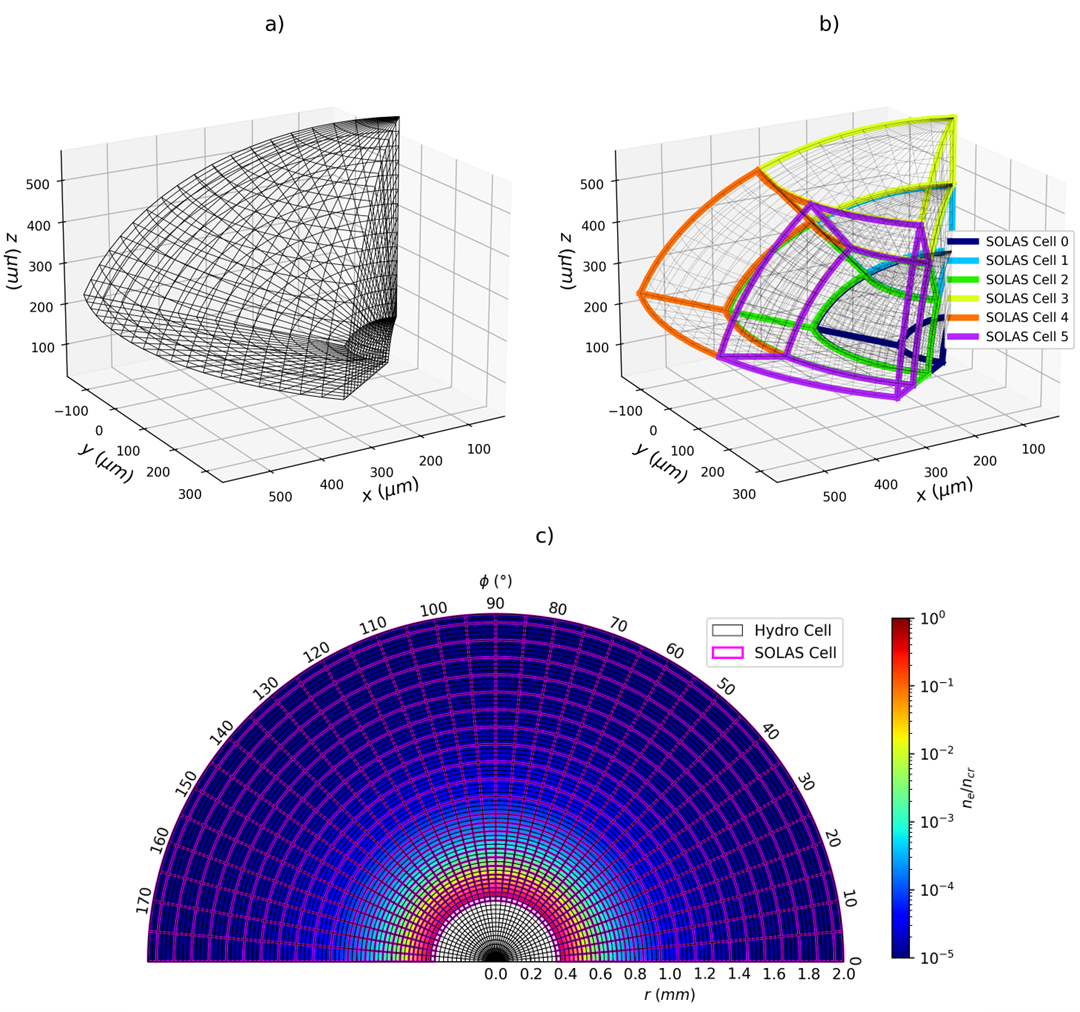
\includegraphics[width=16cm]{Numerics/Images/solas_cells_3imagescombined.png}
    \centering
    \caption{Illustrative diagrams demonstrating a) the spherical polar mesh used by \textsc{Chimera} for hydrodynamic calculations, b) the cell combination mechanism employed by \textsc{Solas} to obtain a roughly equal area grid for spherical simulations and c) the adaptive radial cell combination to reduce resolution in regions where \ac{CBET} and refraction are unimportant.}
    \label{fig:SOLAS_combined_cells}
\end{figure}

Ideal \ac{ICF} experiments are spherically symmetric and departures from this symmetry are usually next-order corrections to a spherical implosion.
Simulations of these experiments therefore typically employ a computational grid with spherical symmetry.
\textsc{Chimera} typically simulates direct-drive implosions with a spherical-polar Eulerian mesh, shown in figure \ref{fig:SOLAS_combined_cells}.a.
This grid has the advantage of simplicity to take gradients across cells and develop new physics modules for the code, however it has the disadvantage that cell edge lengths go to zero as the radial coordinate, $r\rightarrow 0$ and the polar coordinate, $\theta\rightarrow 0,\pi$.
This limits the hydrodynamic timestep as stable explicit timesteps are inversely proportional to edge lengths, increasing the cost of 3D spherical simulations.
The issue is circumvented at late times in the implosion by remapping onto a Cartesian grid, which does not have vanishing edge length and face areas \cite{chittenden_signatures_2016}.

Computing \ac{CBET} however required at least a single ray from each interacting beam to pass through each computational grid cell where the interaction should be important.
For spherical-polar meshes the vanishing cell volume therefore sets extreme minimum ray number limits for the calculation to fully resolve all the fields, especially for direct-drive simulations due to the requirement to resolve the reflected fields which spread out over $4\pi$ steradians, as is shown in figure \ref{fig:reflectedrays}.
Hydrodynamic resolutions are often also excessive for ray trace calculations to resolve the necessary refraction and energy exchange of the light.
Rays must stop at each cell boundary in order to deposit the correct amount of energy into each grid cell and therefore the expense of the ray trace is directly proportional to the number of grid cells that the rays see.

To circumvent this issue cells can be combined around the spherical grid angles in order to make a semi-structured Eulerian grid, as is shown in figure \ref{fig:SOLAS_combined_cells}.b.
Hydrodynamic grid cells are merged together on the \textsc{Solas} mesh in each grid direction until a pre-speicifed resolution, set by the problem is reached.
In figure \ref{fig:SOLAS_combined_cells}.b, many cells are combined in each direction to clearly display the effect.
Typically for spherical simulations however, the cells are not combined in the polar direction, $\theta$ and $n_{\phi}$ cells are combined in the azimuthal direction until the azimuthal and polar resolutions match, explicitly $n_{\phi}r\Delta\phi\sin\theta \approx r \Delta\theta$ at a given radius, $r$.

Figure \ref{fig:SOLAS_combined_cells}.c demonstrates the capability of the meshing algorithm to adaptively combine cells in the radial direction based upon density gradients.
This allows large cells to exist in the coronal plasma where the light refracts minimially and deposits little energy, while the sharp turning point regions close to the critical surface can be well resolved.
To find the number of radial cells to combine at a given radius, the cell combination algorithm varies on the number of cells to combine $n_r$ and calculates the maximum gradient length scale from all combined hydrodynamic cells, $L_{n_e}=n_{crit}/|\nabla n_e|_{\max}$.
The algorithm then finds the optimal number of cells to merge together such that the new cell resolution $n_r\Delta r \approx C_L L_{n_e}$, where $C_L$ is a user parameter\footnote{Default value set to $C_L=0.05$.} which can be reduced to limit cell combining.
A maximum cell size is also set to prevent excessively large cells in regions with minimal density gradients.

Note that many options for equal area computational grids exist which, unlike the semi-structured grid described here, are completely uncorrelated from the hydrodynamic mesh \cite{cheong_eigensolutions_2015,malkin_new_2019}.
These have the advantage that the grid can be completely chosen based solely upon the laser ray trace.
However, the mesh described in this section has the advantage that interpolation to the hydrodynamic mesh is extremely straightforward as the \textsc{Solas} grid cells completely overlap the \textsc{Chimera} cells.
This also removes minimises artefacts from interpolation between the grids, which have the potential to introduce spurious high order modes to the deposition source term.

%################################################################################
%################################################################################
\subsection{Ray Initialisation}
\label{sec:SOLAS_ray_init}

\begin{figure}[t!]
    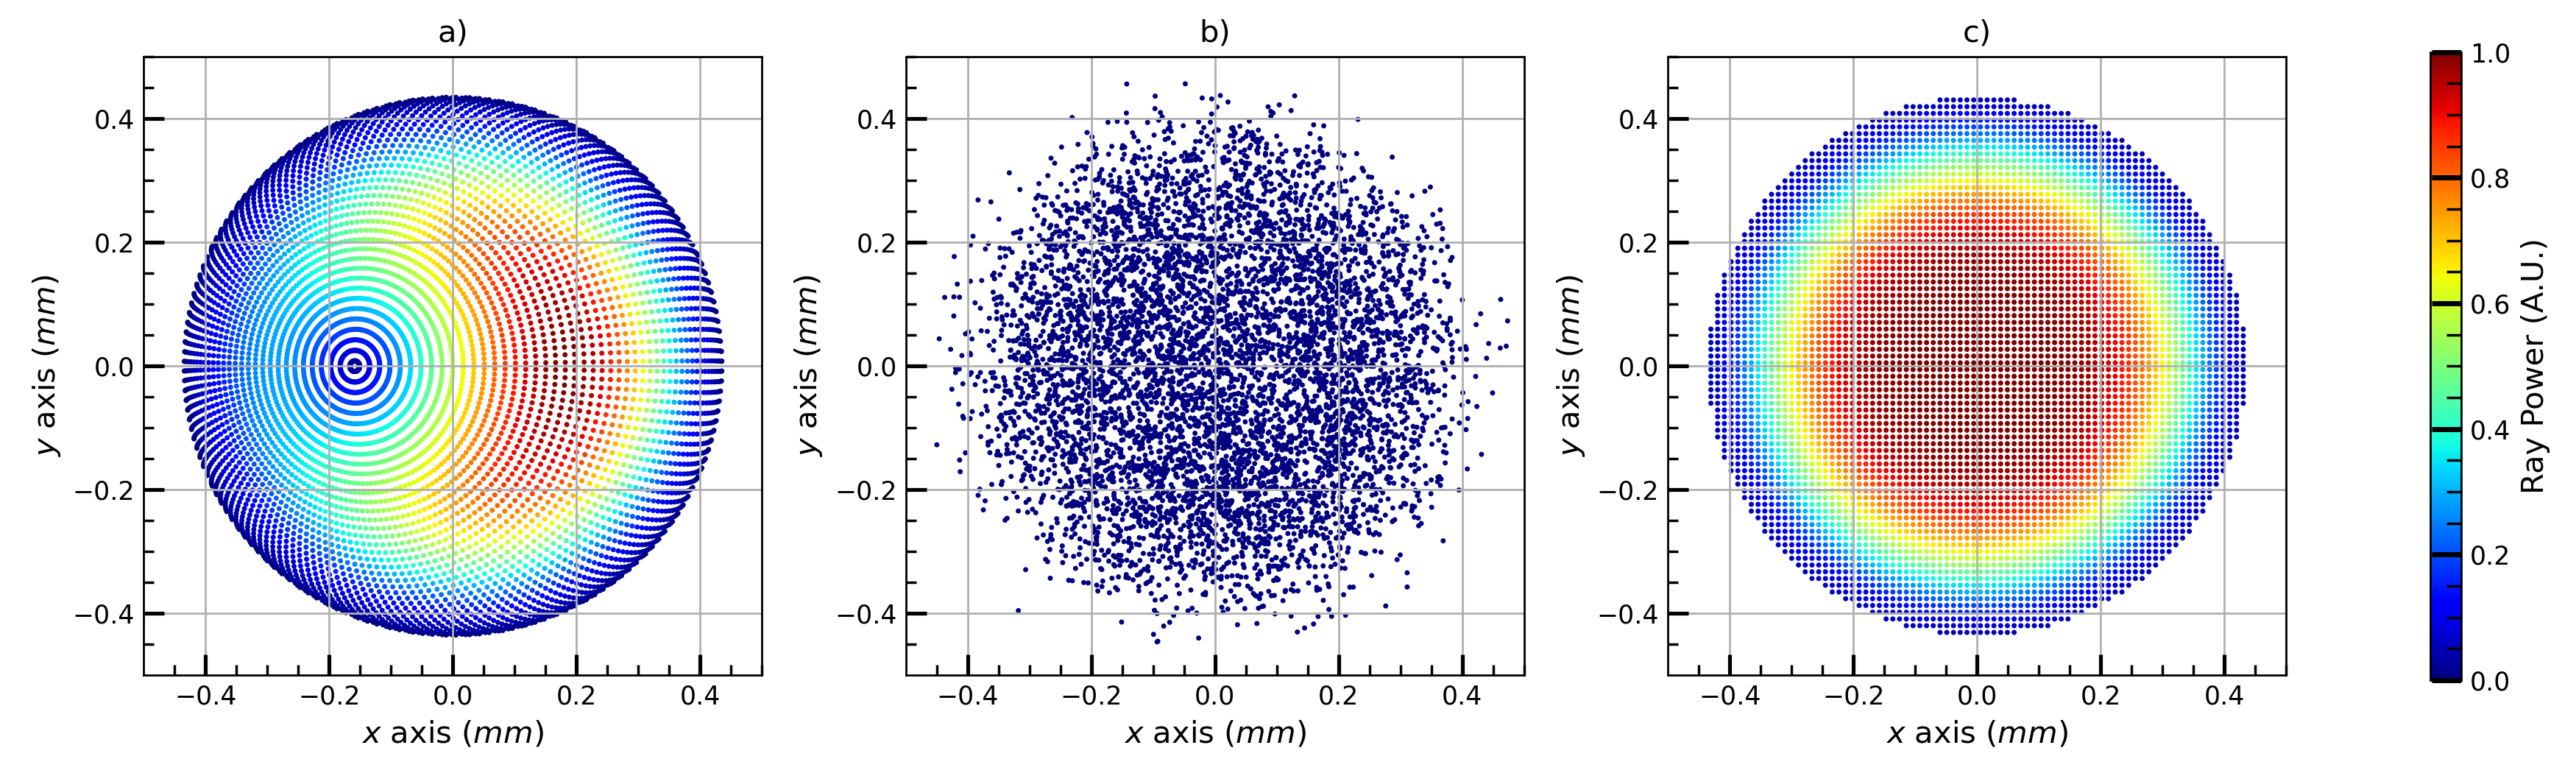
\includegraphics[width=14.5cm]{Numerics/Images/ray_init_plots.png}
    \centering
    \caption{Example initial locations for $\sim4000$ rays for an OMEGA beam port with super-Gaussian intensity profile, with a shape defined by $n_s=5.2$ and $\sigma=352\ \mu m$.
    The inverse-projection ray locations are shown in sub-figure a) which demonstrate a higher ray density for rays pointed to the pole at $x\sim\  -0.15 mm$.
    b) shows the randomly sampled rays where all rays are initialised with the same power, and c) shows uniformly sampled rays.}
    \label{fig:SOLAS_ray_init}
\end{figure}

To obtain a noise-free energy deposition source term from a ray trace, both the grid and choice of initial rays number and location is crucial.
The problems are closely related as a higher resolution grid will require a larger density of rays to get an equivalent ray-per-cell statistics.
It is therefore wise to choose the number of rays used in a simulation to be some function of the grid used for the ray-trace.
Several methods for ray initialization which have been implemented shall be briefly outlined here, along with a summary of their strengths and weaknesses.

All beams profiles described in this thesis have circularly symmetric super-Gaussian intensity profiles described by the equation,

\begin{equation}
    \label{eq:supgaus}
    I(r) = I_0 \exp{\Bigl( -\Bigl| \frac{r}{\sigma} \Bigr| ^{n_s} \Bigr)},
\end{equation}

where $r$ is the distance from the centre of the beam port, perpendicular to the beam normal, $I_0$ is the peak intensity, $\sigma$ is the beam width\footnote{The radius at which $I=I_0e^{-1}$.} and $n_s$ is the super-Gaussian exponent.

\paragraph*{Uniform Sampling}
In this method of ray initialisation, demonstrated in figure \ref{fig:SOLAS_ray_init}.c, each beam is assigned a number of rays and a maximum ray initialisation width\footnote{The maximum initialisation width is usually set to be the radius at which $I=I_0e^{-3}$.}, beyond which rays are not initialised.
Rays are then placed in a uniform, square grid on this plane with a power proportional to the intensity value from by equation \ref{eq:supgaus} and removed if their intensity is below $I_0e^{-3}$, which gives the ray convex hull in \ref{fig:SOLAS_ray_init}.c the circular shape.
For all three procedures described in this subsection, the total summed power of the rays is normalised to the incident beam power after the initialisation of all rays is complete.
Typically, for direct-drive, the total number of rays used for spherical simulations is chosen to be,

\begin{equation}
    \label{eq:SOLAS_nray_uniform}
    N_{ray} = C_{N}\max{(N_r N_{\phi},N_r N_{\theta},N_{\theta} N_{\phi})},
\end{equation}

where $N_{i=r,\phi,\theta}$ is the number of \textsc{Solas} grid cells in that grid direction and $C_N$ is a user-parameter multiplier which to give better ray statistics for CBET simulations when required.
$C_N\sim 2$ is found to give converged deposition when including \ac{CBET} and so this value is used by default.

When there is sufficiently low ray-per-cell statistics, beat phenomena can occur between the ray spacing and the grid resolution.
In this event, especially when using a nearest neighbour interpolation for ray power deposition onto the grid, significant spurious modes can be introduced to the power deposition.
To resolve this, ray locations can be `dithered' so that they take a random position within the polygon\footnote{This polygon is a square for uniform sampling, but not for inverse-projection}, defined by neighbouring ray locations.
This option is always used for simulations using uniform sampling in this thesis.

\paragraph*{Random Sampling}
Rays can also be randomly sampled according to the intensity profile.
Example ray locations from this method are shown in figure \ref{fig:SOLAS_ray_init}.b.
Note that the intensity profile purely emerges from the ray locations in this method as all rays have equal power.
For no \ac{CBET} simulations this is a useful method as it minimises coherent build-up of noise from ray-spacing, grid-resolution beating.
However, the wings of the intensity profile have very poor ray statistics so for direct-drive \ac{CBET} calculations, resolving the reflected field and therefore the dominant backscatter \ac{CBET} is excessively expensive.

\paragraph*{Inverse-Projection}
Inverse-projection, is a final method that has been implemented for ray initialisation in \textsc{Solas}.
The algorithm is described in detail in Appendix A of Ref. \cite{marozas_wavelength-detuning_2018}, but is not used for simulations in this thesis and therefore shall only be cursively outlined.
Briefly, the method works by finding several surfaces, defined by fractions of the critical density and then creating aim points in each cell on the surface.
These aim points and their associated area on the surface are back-projected onto each beam port and rays are created if the aim point is not obscured by the surface on which it was created.
The power of the ray is then the back-projected area multiplied by the intensity at the beam port location.
For a spherical polar grid, this gives a ray distribution which varies in ray density according to which region on the beam port maps to regions on the grid with higher or lower cell-face areas.
The rays in the higher ray density at the beam port region which maps to the polar region of the grid, at $x\sim -0.16\ mm$ on figure \ref{fig:SOLAS_ray_init}.a have a correspondingly lower power compared to rays at equal radii to give the same intensity.

While inverse-projection does guarantee good ray statistics at given surfaces for the inbound component of the field, the algorithm does not extend to beyond ray caustics, or the reflected field component.
Therefore, ray statistics are not guaranteed to be good for the reflected field, so the advantages of this method are not evident for direct-drive \ac{CBET} simulations when backscatter must be resolved.
However, for no \ac{CBET}, direct-drive simulations, this is a useful option for ray initialisation.

\paragraph*{}
For all simulations in this thesis, the uniform sampling method with ray dithering is used.
This method is found to give the best ray-per cell statistics across the semi-structured Eulerian grid described in section \ref{sec:SOLAS_mesh} while minimising the overall number of rays used required to resolve \ac{CBET}.

After rays are initialised on each of the beam ports, rays are extrapolated to the edge of the computational domain.
Beam focussing is typically neglected, so all rays are assigned velocities parallel to the beam normal.
This approximation is widely used for codes that simulate OMEGA-scale direct-drive implosions, where the lasers are approximately collimated on the implosion scale \cite{colaitis_inverse_2021,marozas_wavelength-detuning_2018}.
It is assumed that outside of the simulation domain is vacuum and rays are therefore extrapolated to the edge of the computational domain in straight lines, using a simple root finding to find the intersection of the rays with either a spherical, cylindrical or rectangular domain depending on the simulation geometry.

%################################################################################
%################################################################################
\subsection{Equations of Rays and Adaptive Integration}
\label{sec:SOLAS_ray_propagation}

In \textsc{Solas}, each ray is defined by a position $(\mathbf{x})$, wavevector $(\mathbf{k})$, phase $(\phi)$, angular frequency $(\omega)$ and power ($P$).
The partial differential equations that are integrated along the trajectory of each ray for these quantities are,

\begin{equation}
    \label{eq:SOLAS_rays}
    \begin{gathered}
        \frac{d \mathbf{x}}{d \tau}=\mathbf{k}, \\
        \frac{d \mathbf{k}}{d \tau}=\frac{1}{2} \nabla \varepsilon(\mathbf{x}), \\
        \frac{d \varphi}{d \tau}=\frac{\omega}{c} \varepsilon(\mathbf{x}), \\
        \frac{d \omega}{d \tau}=\frac{\omega}{2 c} \frac{\partial\left(n_e / n_c\right)}{\partial t}, \\
        \frac{d P}{d \tau}=-\kappa_{IB},
    \end{gathered}
\end{equation}

where $\varepsilon=1-n_e/n_c$ is the dielectric permittivity of the plasma, $n_e$ \& $n_c$ are the electron \& critical densities, $c$ is the speed of light, $t$ is time, $\kappa_{IB}$ is the \ac{inv-Brem} absorption kernel, given explicitly in equation \ref{eq:inv_brem} and $\tau$ is the ray path length.
The wavevector is normalised such that $|\vec{k}|=\sqrt{\varepsilon}$.
The optical path length is related to the arc length, $ds$ by the variable change $ds=d\tau\sqrt{\varepsilon}$.
In some formulations of the ray tracing equations, the differential equations are written in terms of the arc length \cite{marozas_wavelength-detuning_2018,kaiser_laser_2000}, which is equivalent, but more complicated and without benefit.
The frequency shift of the light is only significant for the work presented in this thesis when calculating \ac{CBET} and is discussed in more detail in section \ref{sec:SOLAS_doppler}, where the equation used to evaluate the right-hand side is given explicitly.
Note that the time, $t$ is not related to the ray path length $\tau$, because an operator split approach is taken to the ray trace, such that the hydrodynamic variables are frozen and the ray trace finds the time independent trajectory of the light through these profiles.
The path length $\tau$ is therefore best seen as a parameterisation of the ray curve.

\paragraph*{Adaptive RK45 Solver}
The default ray evolution algorithm in \textsc{Solas} is to solve Eq. \ref{eq:SOLAS_rays} using an adaptive RK45 algorithm with stepsize control \cite{press_numerical_2007}.
Ray steps are either limited by the error from this algorithm, or by distance to the next impact with a cell face.
Evaluations of the right-hand side of these equations employ trilinear interpolation for $n_e$, $\nabla n_e$ and $T_e$ to obtain varying values for these quantities at different locations throughout the cell.
All other quantities are either defined at the ray location, or use nearest neighbour interpolation.
The \texttt{bspline-fortran} library has also been implemented to allow tricubic interpolation of $n_e$, which yields a quadratically varying $\nabla n_e$ across the grid \cite{williams_bspline-fortran_2024}.
This is slow to evaluate many times per ray step as is required in an RK45 algorithm and therefore limits performance, but is used throughout this chapter as a higher order solution to validate accuracy of the default interpolation.

Linear interpolation of $n_e$ and $T_e$ is required for accurate computation of $\kappa_{IB}$, especially for `cold-start' simulations where light impacts upon a solid target and the plasma profiles have steep gradients.
Interpolation of $\nabla n_e$ was found to be necessary to obtain low-noise ray amplitudes from neighbouring rays for \ac{CBET} evaluation, which is described in more detail in \ref{sec:SOLAS_field_reconstruc}.
Linear interpolation of both $n_e$ and $\nabla n_e$ is technically inconsistent, because $\nabla n_e$ should be the gradient of $n_e$, however the test cases presented in section \ref{sec:SOLAS_ray_validation} found that this did not reduce accuracy compared to the Kaiser algorithm, which employs a self-consistent linear interpolation of $n_e$ and constant $\nabla n_e$ within a computational cell.

\paragraph*{Kaiser Algorithm}
The Kaiser algorithm for ray integration has also been implemented \cite{kaiser_laser_2000}.
In this algorithm, each cell has a single $\nabla n_e$ and an $n_e$ value defined at the cell centre, allowing for linear interpolation of $n_e$ throughout the cell.
In a constant $\nabla n_e$ region, the trajectory of rays can be analytically shown to follow a parabola.
The Kaiser algorithm thus evolves rays over parabolic segments between cells by finding the intersection of the parabola with cell faces, using a root finding algorithm.
Assuming constant $\nabla n_e$ cells leads to discontinuities in $n_e$ at cell interfaces when the true gradient is not linear and thus Snell's Law is used to refract rays upon cell exit.
While this method is often slightly more efficient compared to the adaptive RK45, it was found that when attempting to reconstruct the ray amplitude from the area of neighbouring rays, as outlined in section \ref{sec:SOLAS_field_reconstruc}, excessive noise was introduced in the amplitude from the discontinuous refraction.
Therefore, the adaptive algorithm was used for all work in this thesis, other than where explicitly outlined.

\begin{figure}[t!]
    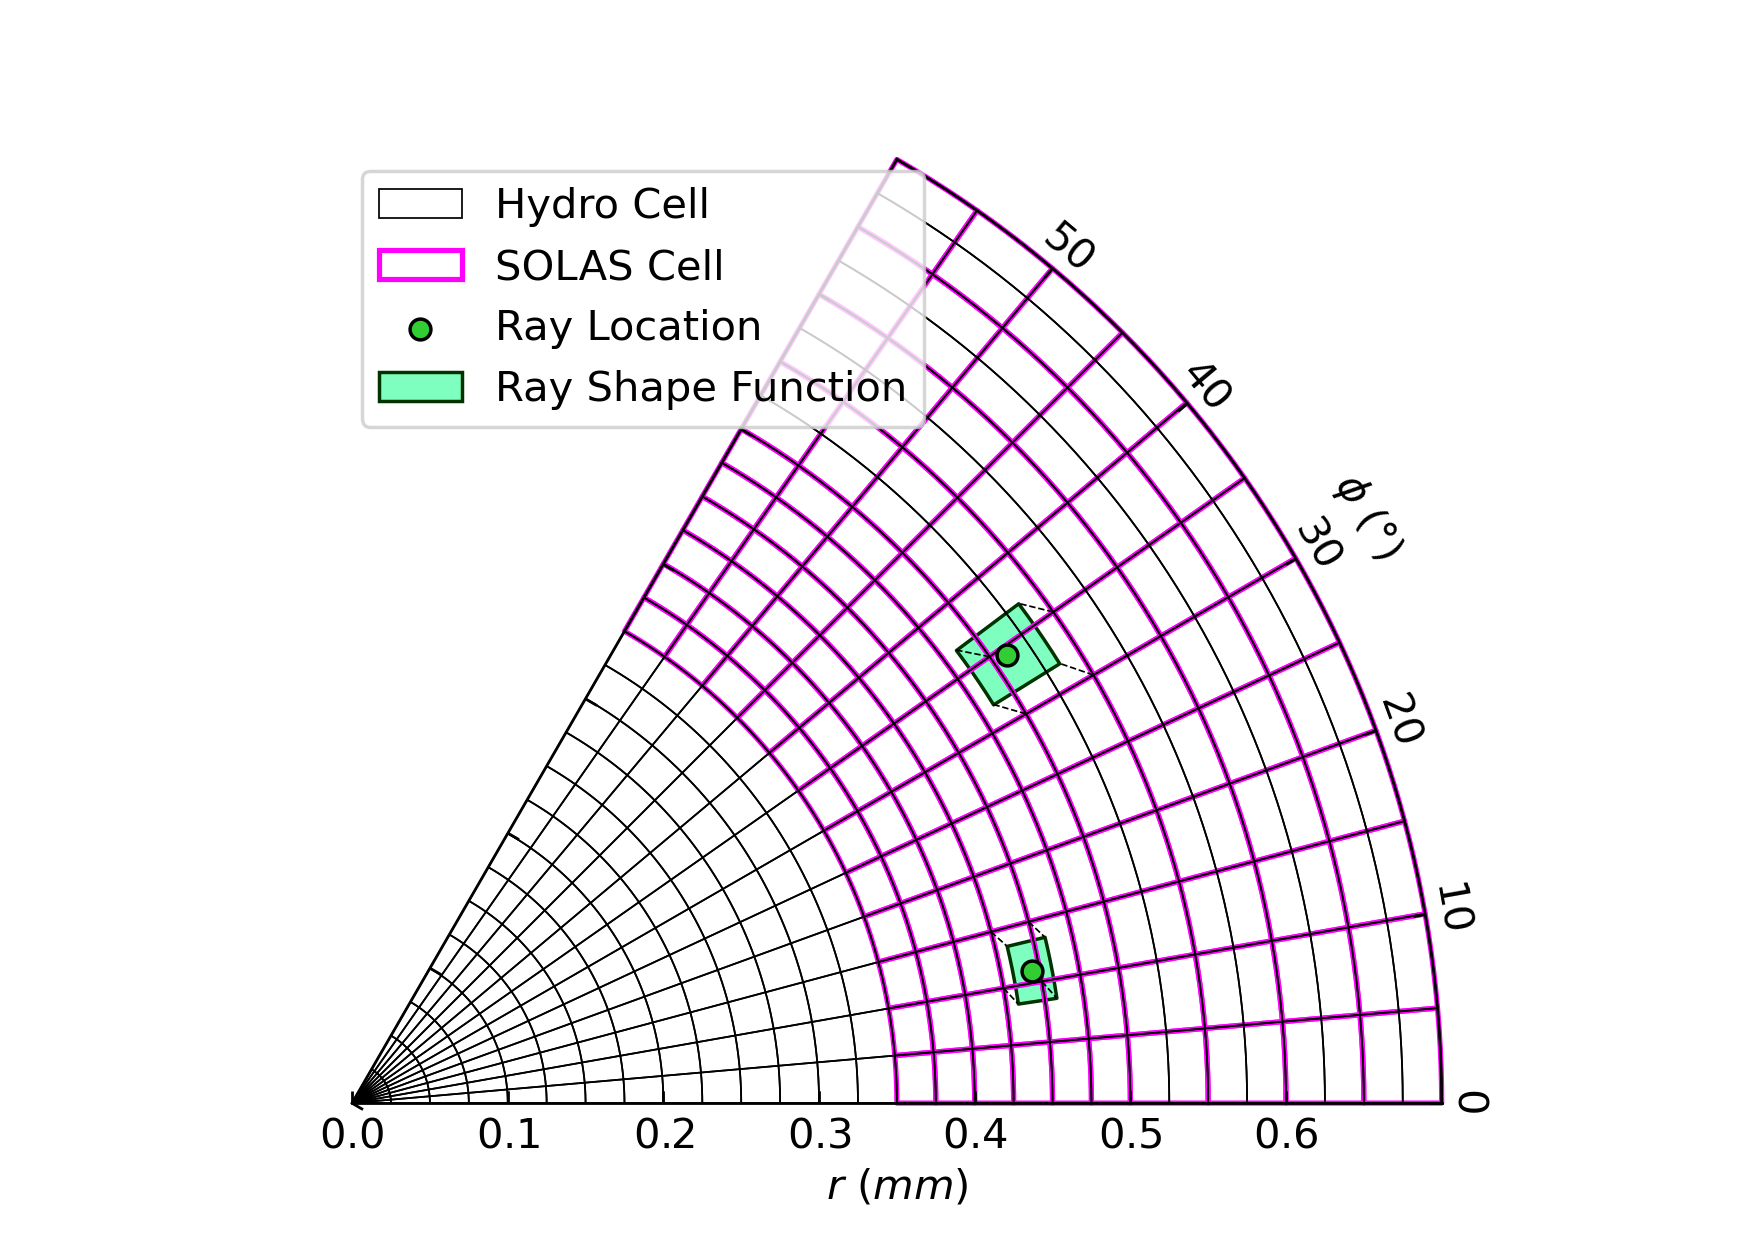
\includegraphics[width=8.0cm]{Numerics/Images/SOLAS_ray_shape_functions.png}
    \centering
    \caption{Demonstration of the shape function smearing weighting for ray power interpolation to the \textsc{Solas} mesh for a cylindrical mesh.
    The shape function has the same size and geometry as the \textsc{Solas} grid cell which the ray is located in.
    A top-hat shape function is used, so the fraction of the deposited power interpolated to a given cell is proportional to the volume overlap of the shape function with the cell.}
    \label{fig:SOLAS_ray_shapefunction}
\end{figure}

\paragraph*{Shape Functions for Ray Deposition}
Nearest neighbour interpolation of power deposition, which is defined along the ray trajectory, onto the computational grid can result in significant levels of noise in the power deposition profile when ray statistics are not sufficiently high.
This is similar to problems experienced in \ac{PiC} codes when interpolating macro particles to the grid without the use of shape functions \cite{birdsall_plasma_1985,arber_contemporary_2015}.
A \ac{PiC}-inspired shape function approach was taken therefore, where the power deposition from rays is smeared across neighbouring cells.
A top hat shape function is used, with a shape function that has the size and shape of the cell that the ray is located within, as is shown in figure \ref{fig:SOLAS_ray_shapefunction}.
The power deposited into each cell that has an overlap with the shape function bounds is therefore proportional to the volume overlap of the shape function with the cell.
This approach is more explicitly outlined, particularly for the case of the non-logically rectilinear grids which are present for \textsc{Solas}, in Ref. \cite{cornet_new_2007}.
This smearing is somewhat numerically diffusive and therefore can be optionally disabled.
For the work presented in this thesis, the shape function smearing is employed for multidimensional direct-drive simulations, but otherwise disabled.

%##################################################
\subsubsection{Ray Solver Validation}
\label{sec:SOLAS_ray_validation}

Several validation problems have been conducted to verify that the ray solver has been implemented correctly.
Here we present the quadratic trough and cylindrical helix test problems which compare the path of a single ray in a density profile to an analytic solution to verify that the ray solvers correctly obtain for the trajectory of light.
The blast wave problem is also presented which is a test of \ac{inv-Brem} absorption to an analytic solution in the absence of thermal conduction and hydrodynamic motion.

\paragraph*{Quadratic trough}

\begin{figure}[t!]
    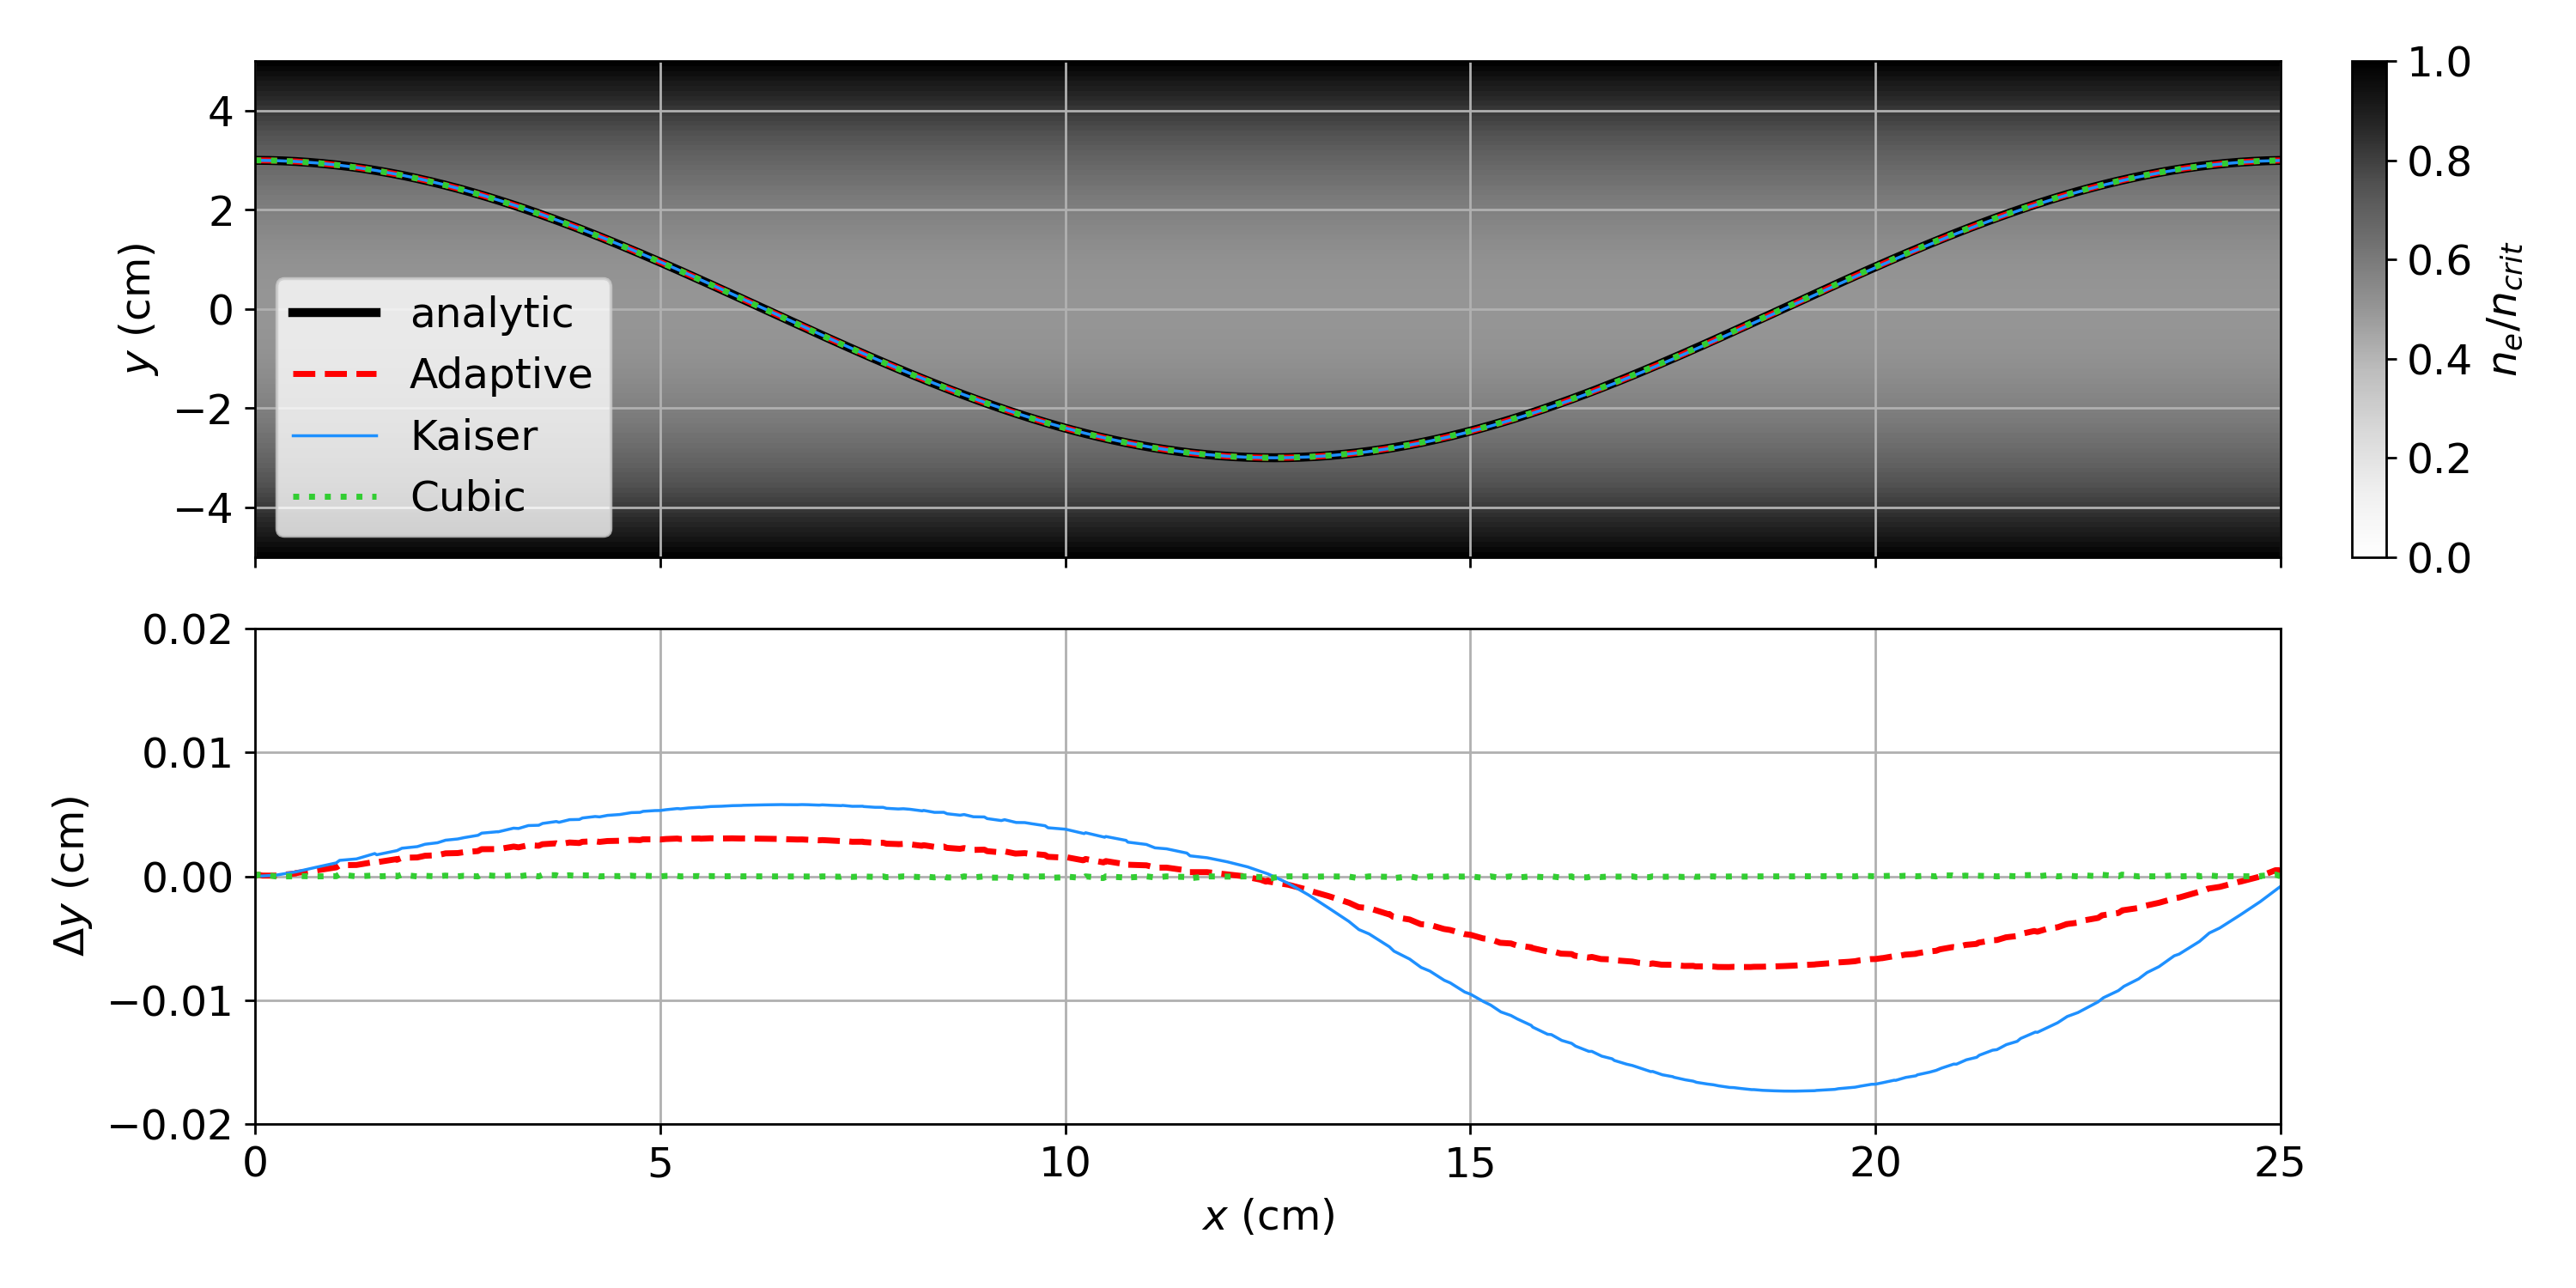
\includegraphics[width=\linewidth]{Numerics/Images/Quadtrough.png}
    \centering
    \caption{This figure demonstrates results of the quadratic trough ray trajectory test problem for the adaptive solver with 3 different cases.
    These are default settings (linear interpolation of both $n_e$ and $\nabla n_e$), the Kaiser algorithm (linear interpolation of $n_e$ and uniform $\nabla n_e$ in a cell) and the adaptive algorithm with tricubic interpolation of $n_e$).
    The top plot shows ray trajectories and analytic trajectory and the bottom plot shows absolute errors for the 3 cases.}
    \label{fig:SOLAS_quadtrough}
\end{figure}

The quadratic trough is a test of ray trajectory in a quadratic density trough, which admits an analytic solution of a periodically oscillating ray \cite{kaiser_laser_2000,haines_coupling_2020}.
The density profile used for the test is defined as,

\begin{equation}
    n_e(y) = \frac{n_c}{2} \left( 1 + \frac{y^2}{y_c^2} \right),
\end{equation}

which for light with wavelength $\lambda=351\ \text{nm}$, is initialised with $n_c = 9.049\times 10^{21} \ \text{cm}^{-3}$ and $y_c = 5 \ \text{cm}$.
The domain has bounds $x \in [0,25]\ \text{cm}$ and $y \in [-5,5]\ \text{cm}$ and a ray enters the domain at $[x_0,y_0]=[0,3]\ \text{cm}$.
Analytic integration of the first 2 lines from Eq. \ref{eq:SOLAS_rays}, yields the analytic trajectory as a function of ray path length , $\tau$,

\begin{equation}
    \begin{gathered}
        x(\tau) = \tau\sqrt{1-\frac{n_e(y_0)}{n_c}}, \\
        y(\tau) = y_0\cos{\left( \frac{\tau}{\sqrt{2}y_c} \right)}.
    \end{gathered}
\end{equation}

The analytic trajectory is compared to the solution from the adaptive solver (using both default interpolation and tricubic interpolation of $n_e$) and the Kaiser algorithm in figure \ref{fig:SOLAS_quadtrough}.
The associated error, defined as the difference in $y$ at a given $x$ is also plotted.
Note that all results were obtained using a grid resolution of $100\times100$ cells.
The top panel demonstrates that all trajectories are identical to the analytic solution by eye.
The corresponding errors show that the tricubic interpolation obtains effectively perfectly recreates the analytic solution and the Kaiser error is slightly more significant compared to the default adaptive error.
The tricubic error is insignificant because the cubic interpolation perfectly recreates the true density profile, so the errors are purely numeric, not due to the resolution.
Errors from the other algorithms would therefore decrease more quickly with increasing resolution as the density profile the ray sees becomes more similar to a quadratic trough.
The error from the default adaptive interpolation (linear interpolation of both $n_e$ and $\nabla n_e$) is lower than that of Kaiser (linear $n_e$ and uniform $\nabla n_e$), indicating that the inconsistent interpolation is not a significant issue for resolving ray trajectories.

\paragraph*{Cylindrical Helix}
Test of refraction in non Cartesian coordinates and also of refraction in directions without gridding.

\paragraph*{Blast wave}
Test of \ac{inv-Brem} absorption.

%###############################################################################################################################
%###############################################################################################################################
%###############################################################################################################################
\section{Ray Based Field Reconstruction and Ray Sheets}
\label{sec:SOLAS_field_reconstruc}

Say that we want to find the field to get CBET.
For rays this means solving the transport equation to get ray amplitude and then using amplitude to get field.
Talk about the concept of ray amplitude and how it can be related to an area of adjacent rays.

%################################################################################
%################################################################################
\subsection{Amplitude Estimate from Neighbour Rays}
\label{sec:SOLAS_ray_amplitude}

Go into detail about how the area is obtained from neighbour rays.
Talk about the concept of sheets and caustics as divergence of amplitude.
Also talk about `Interpolation' from rays to cells and vice versa.

%################################################################################
%################################################################################
\subsection{Caustic Field Capping}
Say that since amplitude diverges in the caustic region, necessary to cap it.
In reality diffraction would limit the field in this region, but standard geometric optics rays can't model diffraction.
Therefore typical approach which we follow is to limit the reconstructed field to a sensible, diffraciton-limited value.

%##################################################
\subsubsection{Field Limiter Approach}
Say that this is the approach used throughout the thesis apart from in some validation problems where it is labelled.
Caps the field to the maximum of a Airy function (ray going up linear density profile).

%##################################################
\subsubsection{Etalon Integral}
This is an improvement which basically allows for deviations from linearity.
This is not used normally, other than when cell size << wavelength, because it needs knowledge of the other sheet from the beam which is present in caustic region.
Could be implemented using linear interpolation.
However, typically we don't have sufficient angular resolution in combined cell grid (at least for 1D hydro) to reliably interpolate sheet to sheet via this grid.
It is generally observed however that the field limiter approach is sufficient.

%################################################################################
%################################################################################
\subsection{Field Reconstruction Validation}
Using Russ' paper with lovely test comparisons to \textsc{Lpse}.
Define the electron density profile here.

%##################################################
\subsubsection{1D Reflected Beam}
Just a simple test of field capping compared to an analytic problem, without refraction.

%##################################################
\subsubsection{2D Reflected Beam}
Same as above, but now for non-normally incident rays, accounting for refraction.
Show test results in both Cartesian and Cylindrical.


%###############################################################################################################################
%###############################################################################################################################
%###############################################################################################################################
\section{Ray Based CBET Model}

Explain that ray based CBET uses the linear gain discussed in theory section.
Say that since this assumes homogineity, effectively applies to small ray steps, which is typically well satisfied.
Also say that this homogeneity within a computational cell and nearest neighbour interpolation of field means that it is not necessary to adaptively integrate the CBET gain.

%################################################################################
%################################################################################
\subsection{Power Change of Rays due to CBET}

Describe how ray energy changes due to CBET from linear gain models (either fluid or kinetic).
Say how when including with inv brem, the deposited power and CBET change must be got carefully (i.e. Marozas paper).

%##################################################
\subsubsection{Fluid CBET Gain}

Breifly discuss the fluid CBET gain and explain why it is easier to use for code validation.

%##################################################
\subsubsection{Kinetic CBET Gain}

Breifly discuss the kinetic CBET gain and why it is better for predictive simulations.

%################################################################################
%################################################################################
\subsection{Dynamic memory structure for storing Fields and CBET Gains}

Give the scaling of storing fields and gains for every beam.
Say that therefore a dynamic memory structure is used which only stores the fields and gain in cells where they are present.
Also state that although the ray trace module must be done in double to numerical errors (e.g. omega differences in resonance and difference between rays), gain is stored as a single which greatly reduces cost.
Give an estimate for how much this reduces the overall memory requirements.

%################################################################################
%################################################################################
\subsection{Doppler Shift of Frequency}
\label{sec:SOLAS_doppler}

Mention time dependant refractive index results in a frequency shift of light.
This is small, however it is significant to include in CBET models as it can shift the resonance.

%################################################################################
%################################################################################
\subsection{Caustic Gain Truncation}

Say that because nearest neighbour interpolation of the fields is used, there exists unphyscial interaction regions where a cell has a field but ray hasn't passed through that portion of the cell.
This problem becomes particularly bad at ray turning points, where a significant amount fo CBET occurs.
Therefore a method called `CGT' is used to effectively enhance the laser grid resolution in the vicnity of caustics.
In cells where a ray from a specific sheet experience a caustic, the field entry for that sheet is divided geometrically, assuming that the caustic is locally a plane.
If a ray from another sheet passes through the cell and is on the `unlit' side of the caustic plane, it will not experience CBET gain.
Ray steps are also limited to the caustic plane.
Other codes have shown that this approach significantly improves energy conservation.

%################################################################################
%################################################################################
\subsection{Coherent Caustic Correction and Caustic Region Identification}

Say how the field reconstruction assumption works everywhere apart from at caustics, where it underestimates the field.
Follow what Russ says in his paper about CC correction and how it significantly improves energy conservation.

%##################################################
\subsubsection{Geometric Approach to identifying the caustic region}

Other codes find caustic region by phase diff and phase interpolation.
We can't interpolate due to resolution issues.
Therefore implemented a new, geometric approach to finding the caustic region.
Talk about how location of rays is stored for each sheet, partitioned by whether they are over or under the amplitude cap.
If a cell has rays from both in a cell, then a plane is found between the two to split the cell into caustic and non-caustic.
If a cell has only capped rays then the whole thing is caustic.
When a ray from another beam passes through, CC mult is applied if in the caustic region.


%################################################################################
%################################################################################
\subsection{Energy Conservation in Ray Based CBET Models}

Talk about how energy is conserved away from caustics when converged.

%################################################################################
%################################################################################
\subsection{Pump Depletion Iterations}
\label{sec:pump_dep_iters}

Talk about why it is necessary to iterate the ray trace.
Mention that it is possible to store ray locations and avoid performing ray trace all over again, but that approach is not taken due to memory limitations.
Talk about convergence parameter.
Mention necessity of damping for complicated, many beam simulations.

%################################################################################
%################################################################################
\subsection{Model Assumptions, Applicability and Validity to ICF}
\label{sec:model_appliciability}

Discuss the key assumptions of the CBET model and whether it is valid to use for LDD and LID.

%################################################################################
%################################################################################
\subsection{Computational Efficency and Scaling}

Talk about how the CBET model is quite expensive.
Give the scaling laws from Russ' paper and explain how that means for many beams, CBET is bound to be the dominant cost in the simulation.
Also say how it shows that memory is a big consideration for CBET models as the gains and fields must be stored.

%################################################################################
%################################################################################
\subsection{\ac{CBET} Validation}
Using Russ' paper with lovely test comparisons to \textsc{Lpse}.
Define the electron density profile here.

%##################################################
\subsubsection{2D \ac{CBET} Without Caustics}
Just a simple test of field capping compared to an analytic problem, without refraction.

%##################################################
\subsubsection{2D \ac{CBET} With Caustics}
\label{sec:SOLAS_CBET_caustic_test}
Same as above, but now for non-normally incident rays, accounting for refraction.
Show test results in both Cartesian and Cylindrical.


%###############################################################################################################################
%###############################################################################################################################
%###############################################################################################################################
\section{Coupling to Hydrodynamics and Example Use}

Here present an entire explanation for the model working coupled to Hydrodynamics.

%################################################################################
%################################################################################
\subsection{Power Deposition}

Say that the deposited power is just added as an energy source to the electrons.
If running in 1D or 2D, it is integrated over other directions first.
Say that when starting from $t=0$, often use a cold-start routine, which uniformly deposits power at the critical surface of a spherical capsule.
This creates an under-dense small region in which the rays can refract and deposit energy.
This is unsatisfactory for imprint simulations, where early time imprinting is important, but that is not considered for this thesis.

%################################################################################
%################################################################################
\subsection{Time step limiter} \label{dtlaser}

Limit timstep based on the fractional electron energy change.
Don't limit timestep in cells far from critical.
This is usually the limitting timestep for `cold start' simulations initially, until deposition begins to occur in hot cells.

%################################################################################
%################################################################################
\subsection{Ray Trace Frequency}

For many beam simulations, such as direct-drive simulations, the laser operator (especially with CBET) is typically one of the more expensive parts of the code.
In the steady state of an implosion, the coronal plasma conditions don't significantly change on the global hydrodynamic timestep.
Therefore the deposition also doesn't change much meaning that previously calculated Pdep can be stored and reapplied on subsequent timesteps.
Especially for CBET simulations, this can reduce runtime by order of magnitude.
Currently the ray trace is performed every timestep up until a pre-specified `warm up' time has expired.
Then the ray trace is performed at a pre-specified frequency by the user.
Experimentation has found that for \textsc{Omega} scale simulations, increasing frequency of calculations doesn't significantly change the answer above ... .

Because LDD pulses often start with a low intensity and then ramp up, CBET gains are also often minimal until late in the implosion.
Therefore field reconstruction and CBET iterations are only performed after a specified start time, normally when the hard-sphere intensity reaches about $1\times 10^{14}$ $Wcm^{-2}$.
CBET iterations are then performed on the laser frequency.

An improved approach shall soon be implemented where laser iterations occur at $dt_{\text{laser}}$ from section \ref{dtlaser}.

%################################################################################
%################################################################################
\subsection{Computational Diagnostics}

Say that a variety of diagnostics can be output.
Qpower with and without CBET.
Geometric intensity.
Electric field (from single or all beams), optionally split into inbound and reflected components, both with and without CBET.

%################################################################################
%################################################################################
\subsection{Example use on \textsc{Omega} Shot 89224}

First briefly describe the shot, showing pulse shape and target.

%##################################################
\subsubsection{1-D Rad-Hydro, 3-D Ray-Trace with CBET Simulation}

Describe the simulation parameters used, e.g. cell resolution, flux limiter etc.
Show the absorbed power vs time and effect of CBET.
Show instantaneuos radial profiles.
Show integrated parameter comparison to \textsc{Lilac} post-shot simulation.
Describe the previous method of tuning, involving a 2D scan of flux limiter and power multipliers.
Say how it's great that the $flim_e = 0.06 \rightarrow 0.15$ and CBET combination now gives a predictive capability for \textsc{Omega} shots.

%##################################################
\subsubsection{3-D Post Process of Absorption Non-Uniformity}

Mention how the model can also be used as a postprocess.
\textsc{Chimera} can restart from 1-D data into spherically symmetric 3-D profiles.
Ray Trace and CBET can then be performed through these profiles to understand the absorption non-uniformity present due to CBET.
Note that comparison of 1-D and 3-D simulations shows that thermal conduction does a good job of smoothing angular deviations in coronal plasma conditions.
The assumption of spherically symmetric profiles for the laser is therefore deemed valid, and it is a technique typically used by post-process CBET codes.

MAYBE??
Mention how ray noise means that we can't use direct deposition.
Therefore use Pdep from field estimate, which is much cleaner.

Talk about how CBET enhances angular non-uniformity.
Show modal decomposition.


%###############################################################################################################################
%###############################################################################################################################
%###############################################################################################################################
\section{Future Model Extensions}

Say that there is even more laser/ CBET physics that is interesting and can be implemented within the raytracing framework.
Some are straightforward to implement, while others more difficult and computationally expensive.

%################################################################################
%################################################################################
\subsection{Langdon Effect on Abosprtion}

Describe Langdon from a kinetic perspective and why it reduces absorption.
Describe how you can fit it and include as a modification to ray tracing absorption if you have the field/ intensity.
Describe the magnitude of the effect for ICF like conditions.
Describe breifly how it would be implemented, say it would not be difficult.

%################################################################################
%################################################################################
\subsection{Langdon Effect on CBET}

Describe what this is.
Say that it is important for high overlapping intensities, eg hohlraum LEH.
Say that it is thought to stabilise the CBET interaction in indirect drive configurations and remove the need for artificial clamps.
Describe breifly how it would be implemented, say it would not be difficult.

%################################################################################
%################################################################################
\subsection{Polarised CBET}

Describe how ion accoustic waves are driven by beat between electric fields from light and therefore is polarisation dependent.
Say how on OMEGA, RPP smoothing means that each beam is split into 2 sub-beams with linear polarisation.
Say that these do not have a symmetry to the configuration about the sphere.
Say that this leads to mode-1 on OMEGA.
Say that you can track polarisation of rays and trace these sub-beams independently.
Would make it more expensive, but definitely feasible.

%################################################################################
%################################################################################
\subsection{Bandwidth for CBET Mitigation Studies}

Describe how bandwidth should reduce LPI growth rates.
Understanding the desired bandwidth to mitigate CBET is a key consideration for design of future laser sysytems.
Fields can be modified to include discrete wavelengths to model bandwidth.

%################################################################################
%################################################################################
\subsection{Additional LPIs}

Could look at TPD, SBS and SRS.
In theory not a difficult problem to do backscatter, but side-SRS is difficult, because additional rays would need to be launched.
This could make the model more useful to indirect-drive experiments and design of ignition scale direct-drive facilities, where SRS is thought to be important energetically due to long scale lengths.



%###############################################################################################################################
%###############################################################################################################################
%###############################################################################################################################
\section{Conclusions}

Say that the chapter has described the validity and implementation of \textsc{Solas} and validated it.
Culminated in demonstrating that the model can reproduce post-shot simulations of an \textsc{Omega} shot from the \textsc{Lilac} code which includes a CBET model.
This demonstrates that the \textsc{Chimera} code now has a predictive capability for \textsc{Omega} scale direct drive experiments, as no free parameter tuning was required.
